%----------------------------------------------------------------------------
\chapter{Evaluation}
%----------------------------------------------------------------------------
This chapter presents the applicability of the designed framework, evaluates its current capabilities and points out improvement possibilities. Section \ref{sec_theoeval} evaluates the current state of the framework, then Section \ref{sec_casestudy} presents a case study about the applicability of our solution. Lastly, Section \ref{sec_futurework} presents the opportunities for the continuation of the work.

%----------------------------------------------------------------------------
\section{Case Study: Pedestrian Crossing} \label{sec_casestudy}
%----------------------------------------------------------------------------
This section demonstrates the capabilities and limitations of the framework. It presents a problem commonly modeled using state-based models, which is complex enough to demonstrate all aspects of the designed Interactive Learning Entity, but also simple enough to solve - thus verify - only using some background knowledge and common sense. [TODO ref gamma tutorial?]

%---------------------------------------------------------------
\subsection{Introduction} \label{subs_casestudyintro}
%---------------------------------------------------------------

The problem to solve is modeling a pedestrian crossing with a standard traffic light and a pedestrian light as illustrated on Figre \ref{fig_casestudy_systemstates}. As the traffic lights and the pedestrian lights on the opposite sides of the crossing behave identically, we are going to model only one instance of each device. 

The traffic light is looping through the red-green-yellow-red sequence. As an extra, there is an interrupted mode that may be triggered by the police, which results in blinking yellow light. The pedestrian light loops through the red-green-red sequence, and turns black when an interrupt arrives. A subsequent interrupt turns the lights back on, also considering that the sytem must always be in a safe state - i.e. the lights must not allow passage for both the pedestrians and the road vehicles at the same time.

\begin{figure}[!ht] 
	\centering
	\fbox{
		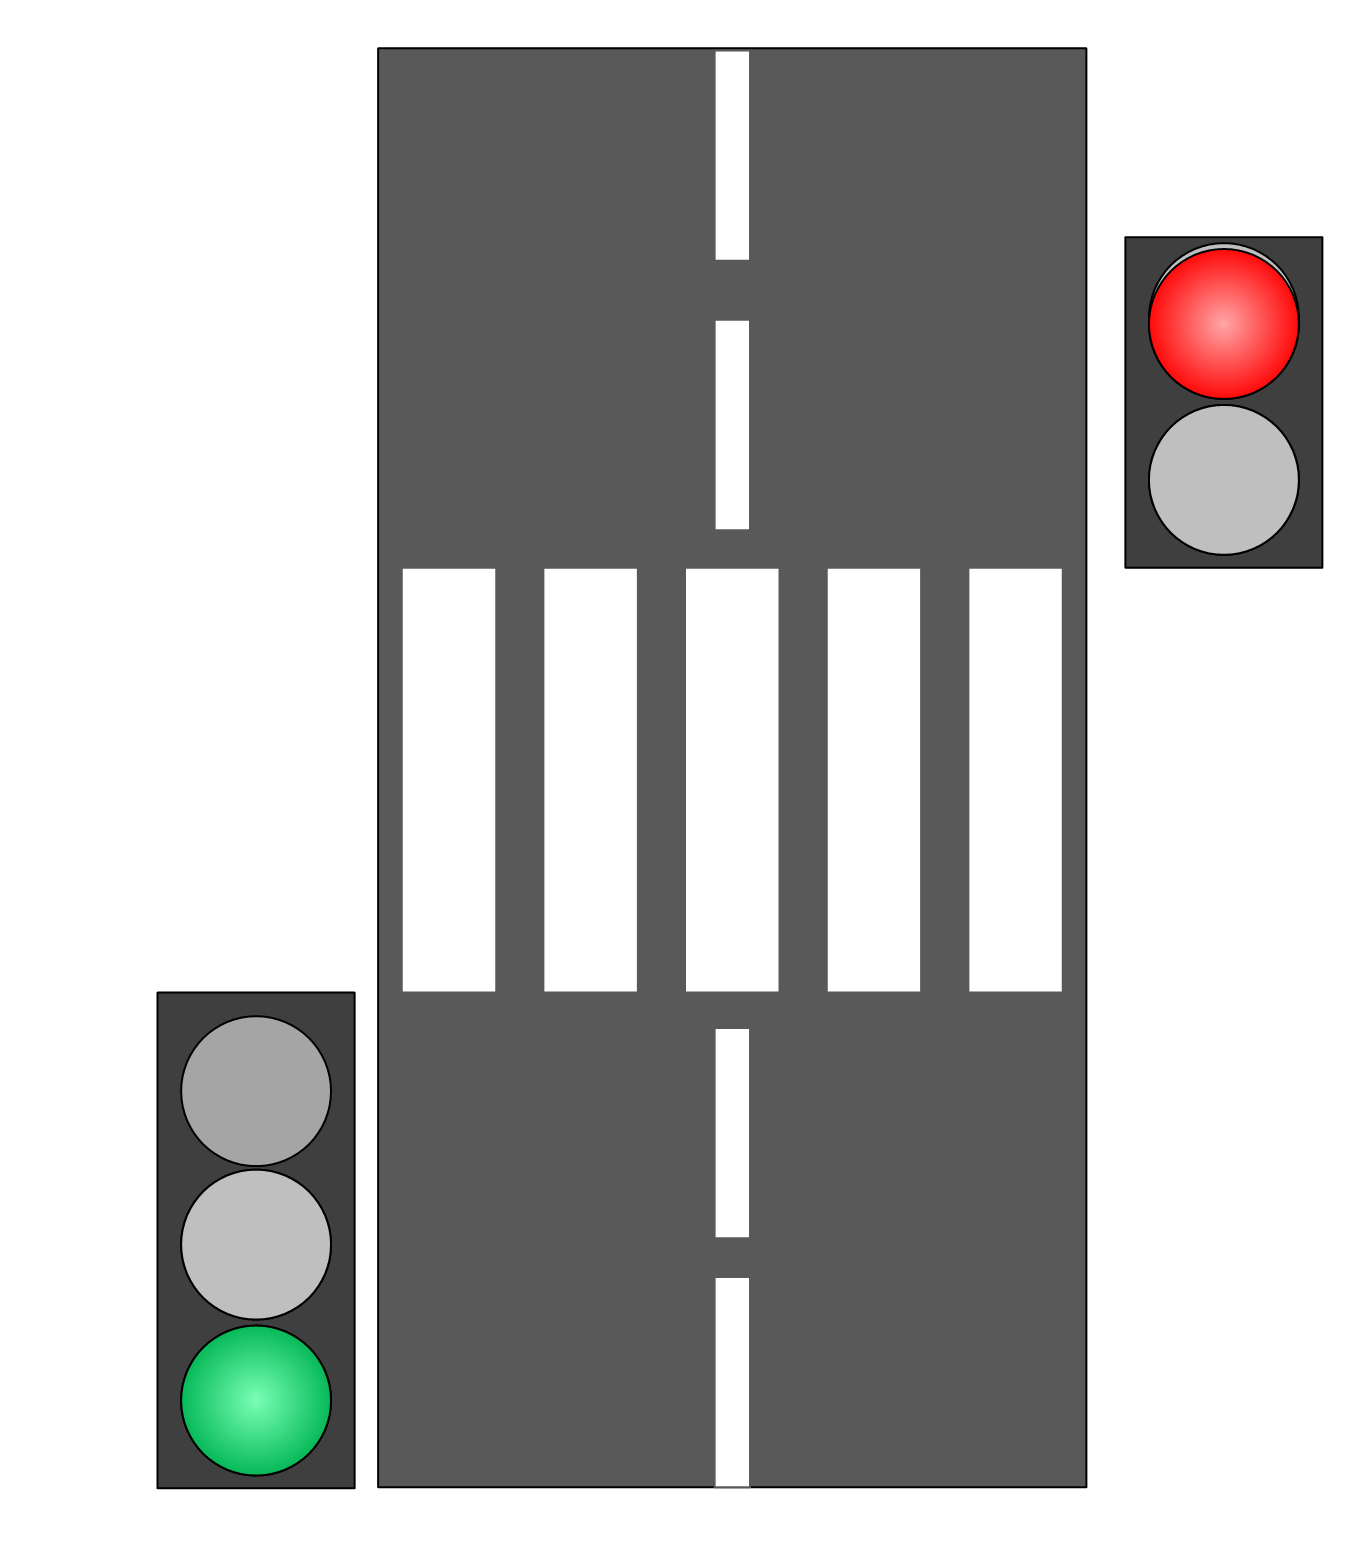
\includegraphics[width=30mm, keepaspectratio]{figures/casestudy_state1.png}
	}
	\fbox{
		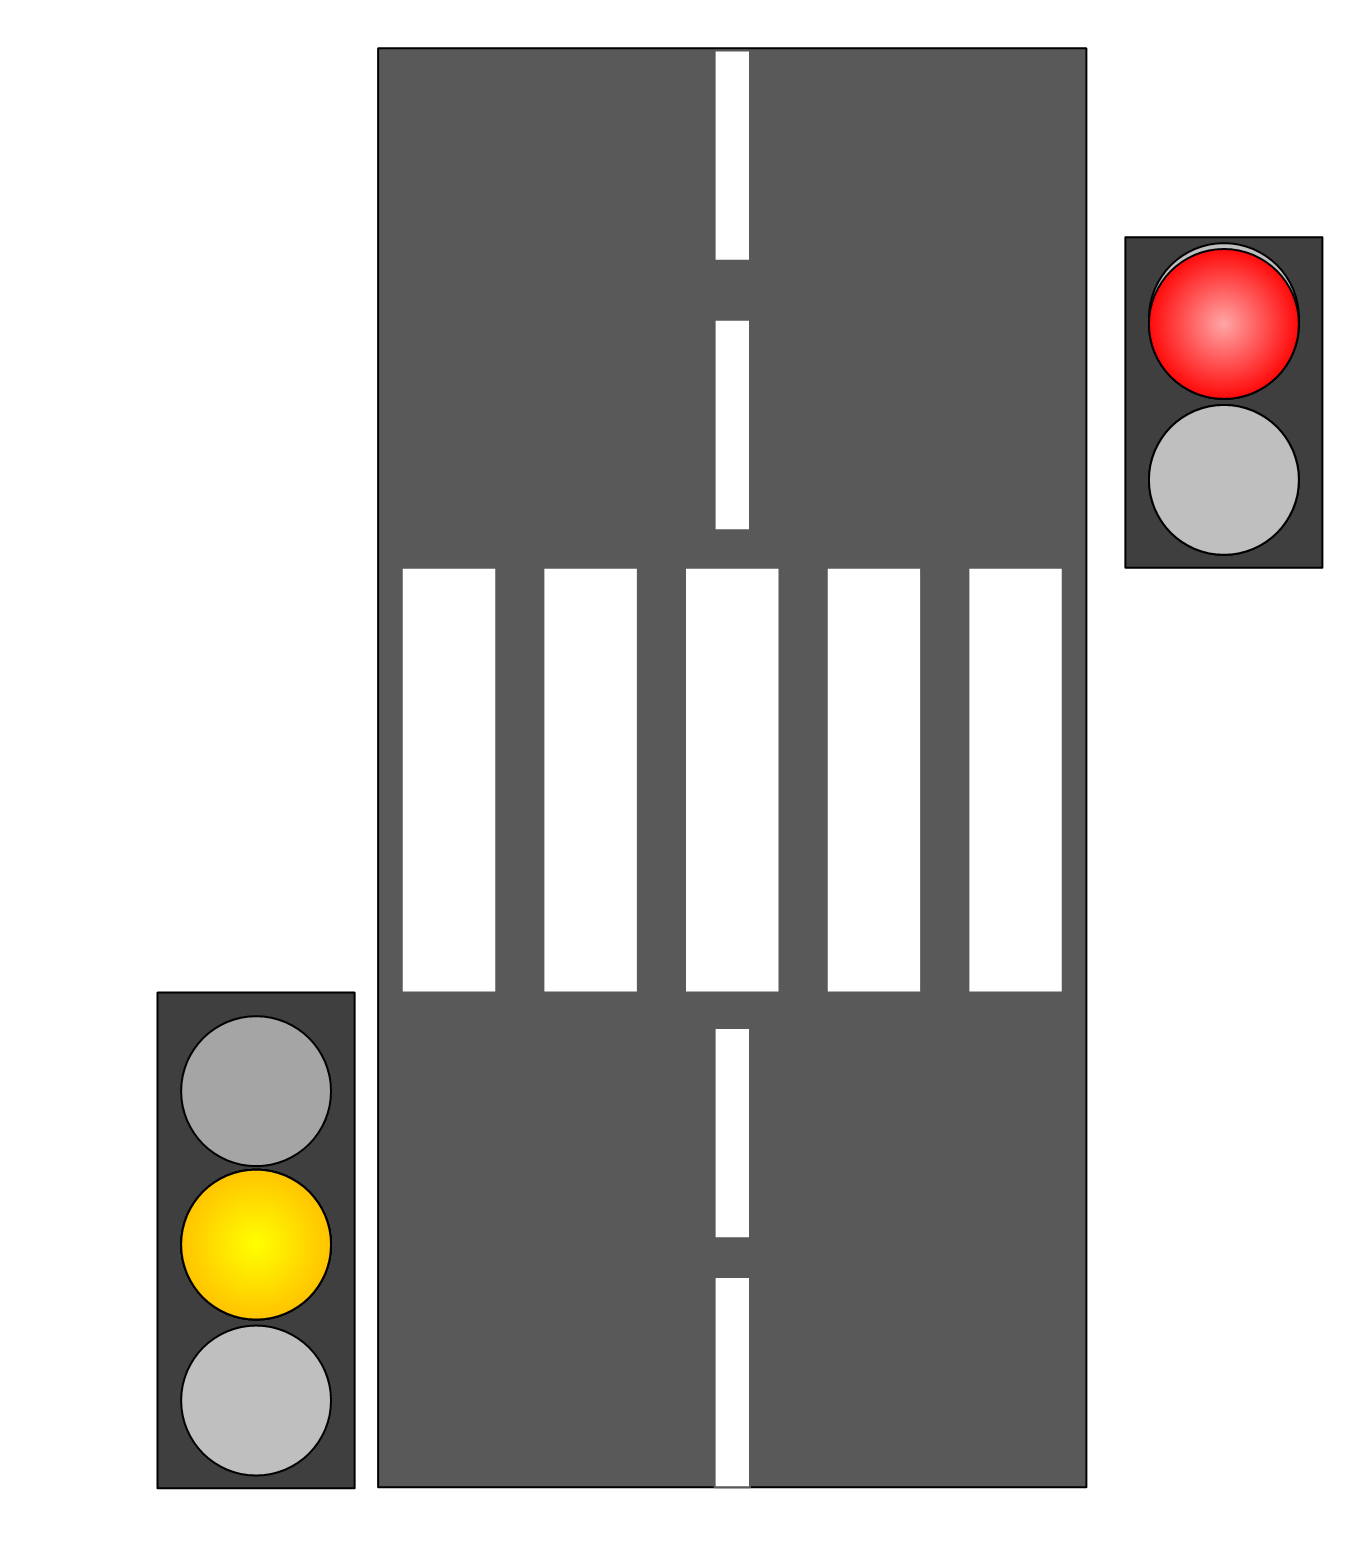
\includegraphics[width=30mm, keepaspectratio]{figures/casestudy_state2.png}
	}
	\fbox{
		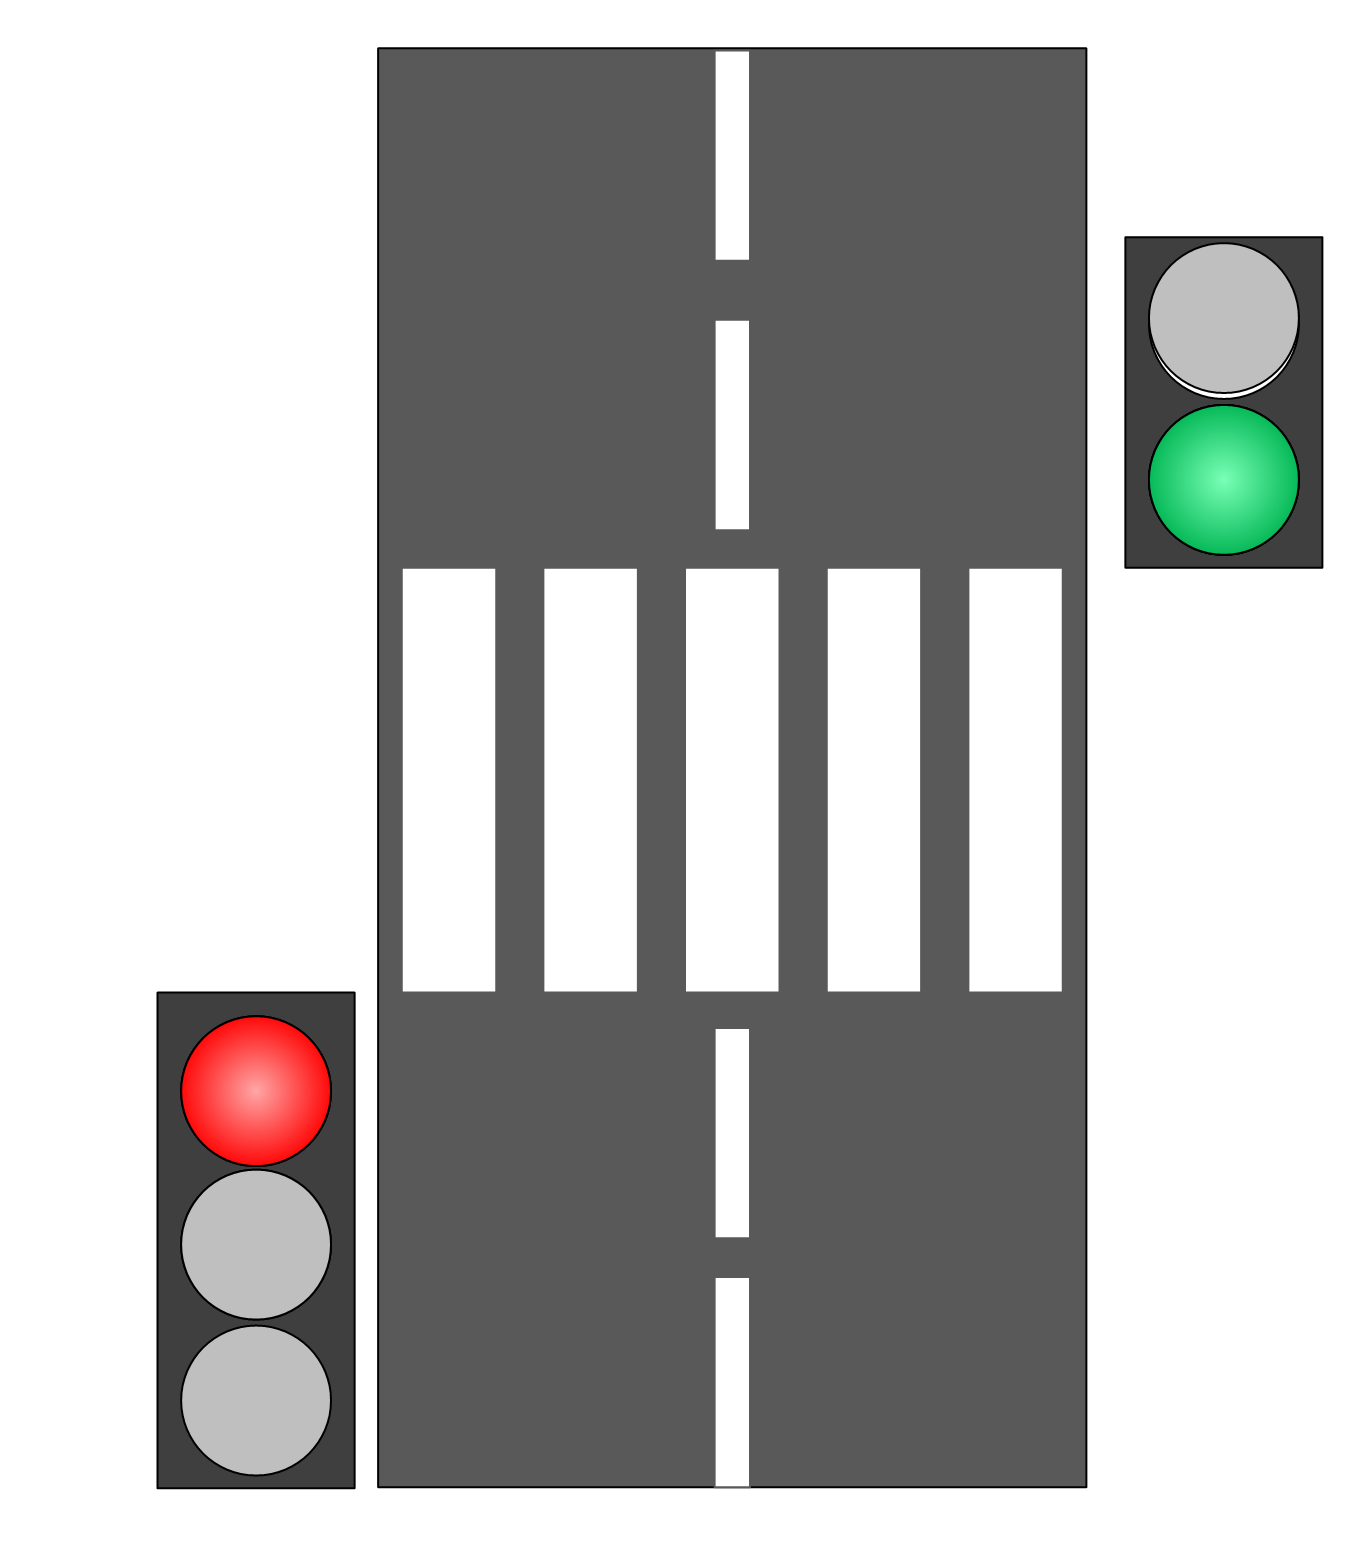
\includegraphics[width=30mm, keepaspectratio]{figures/casestudy_state3.png}
	}
	\fbox{
		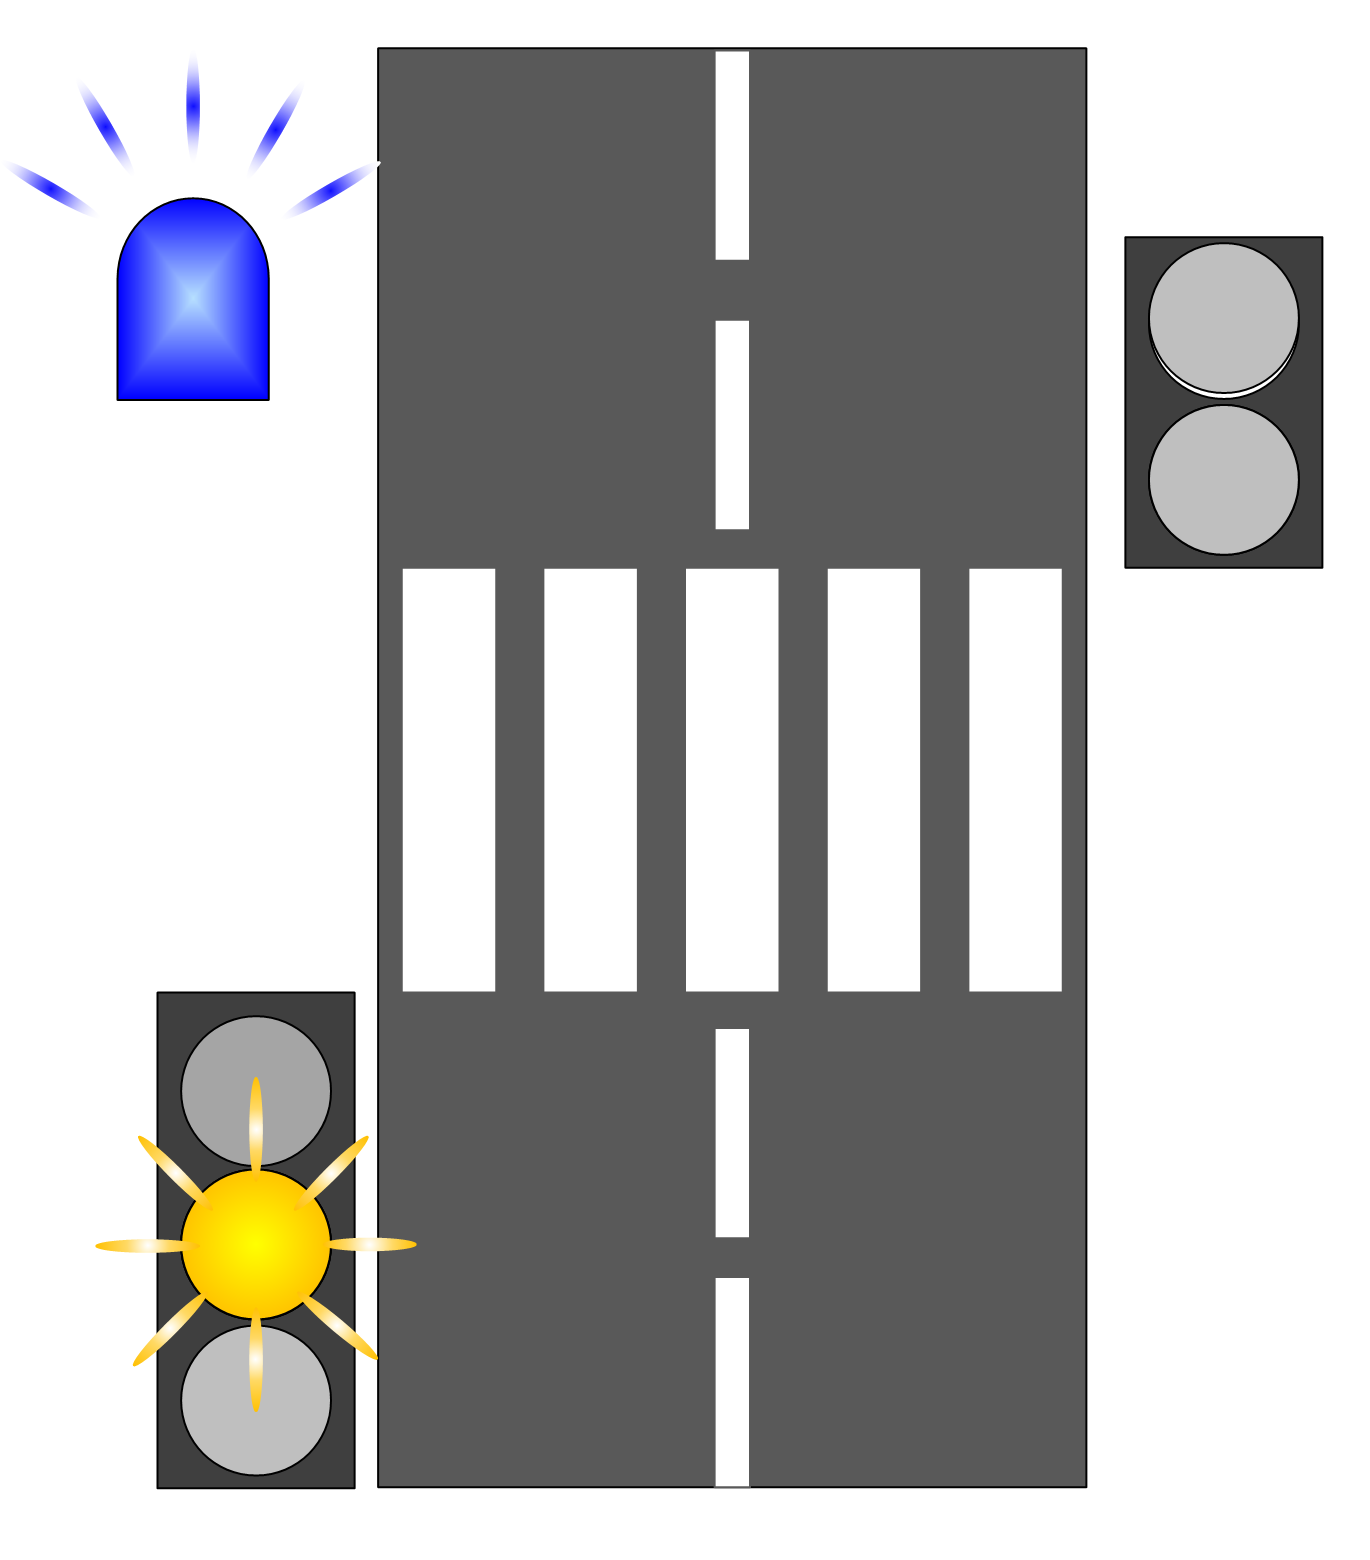
\includegraphics[width=30mm, keepaspectratio]{figures/casestudy_state4.png}
	}
	\caption{Possible states of the system: normal operation (\textit{three from the left}) and the interrupted state \textit{(right)}} 
	\label{fig_casestudy_systemstates}
\end{figure}

%---------------------------------------------------------------
\subsection{Component Design} \label{subs_casestudycomps}
%---------------------------------------------------------------

The previous subsection mentioned two components of the composite system: a traffic light and a pedestrian light. To realize the safe state of the system, the components must synchronize their behavior, justificating the existence of a third, controller component. The traffic and pedestrian light components should have one input and one output port -- they  are relatively simple -- and the controller should have an input port for the police and two output ports for the components.

\textbf{The traffic light component} has two possible inputs on its input port (TrafficControl) - toggle and interrupt - and four outputs on its output port (TrafficDisplay) - red, green, yellow and blinking yellow - as it appeared in the problem description.

\textbf{The pedestrian light component} has the same two inputs on its input port (PedestrianControl) - toggle and interrupt - and three outputs on its output port (PedestrianDisplay) - red, green, and black - as it appeared in the problem description.

\textbf{The controller component} controls the rhythm of the change of states and also interrupts the other components when the police interrupt arrives. It has an input port ('\textit{Police}') for the police interrupt and two output ports ('\textit{TrafficControl}' and '\textit{PedestrianControl}') - matching the input ports of the other components.

The described components and their connections are illustrated on Figure \ref{fig_casestudy_blockdiagram}.

\begin{figure}[!ht] 
	\centering
	%\fbox{
		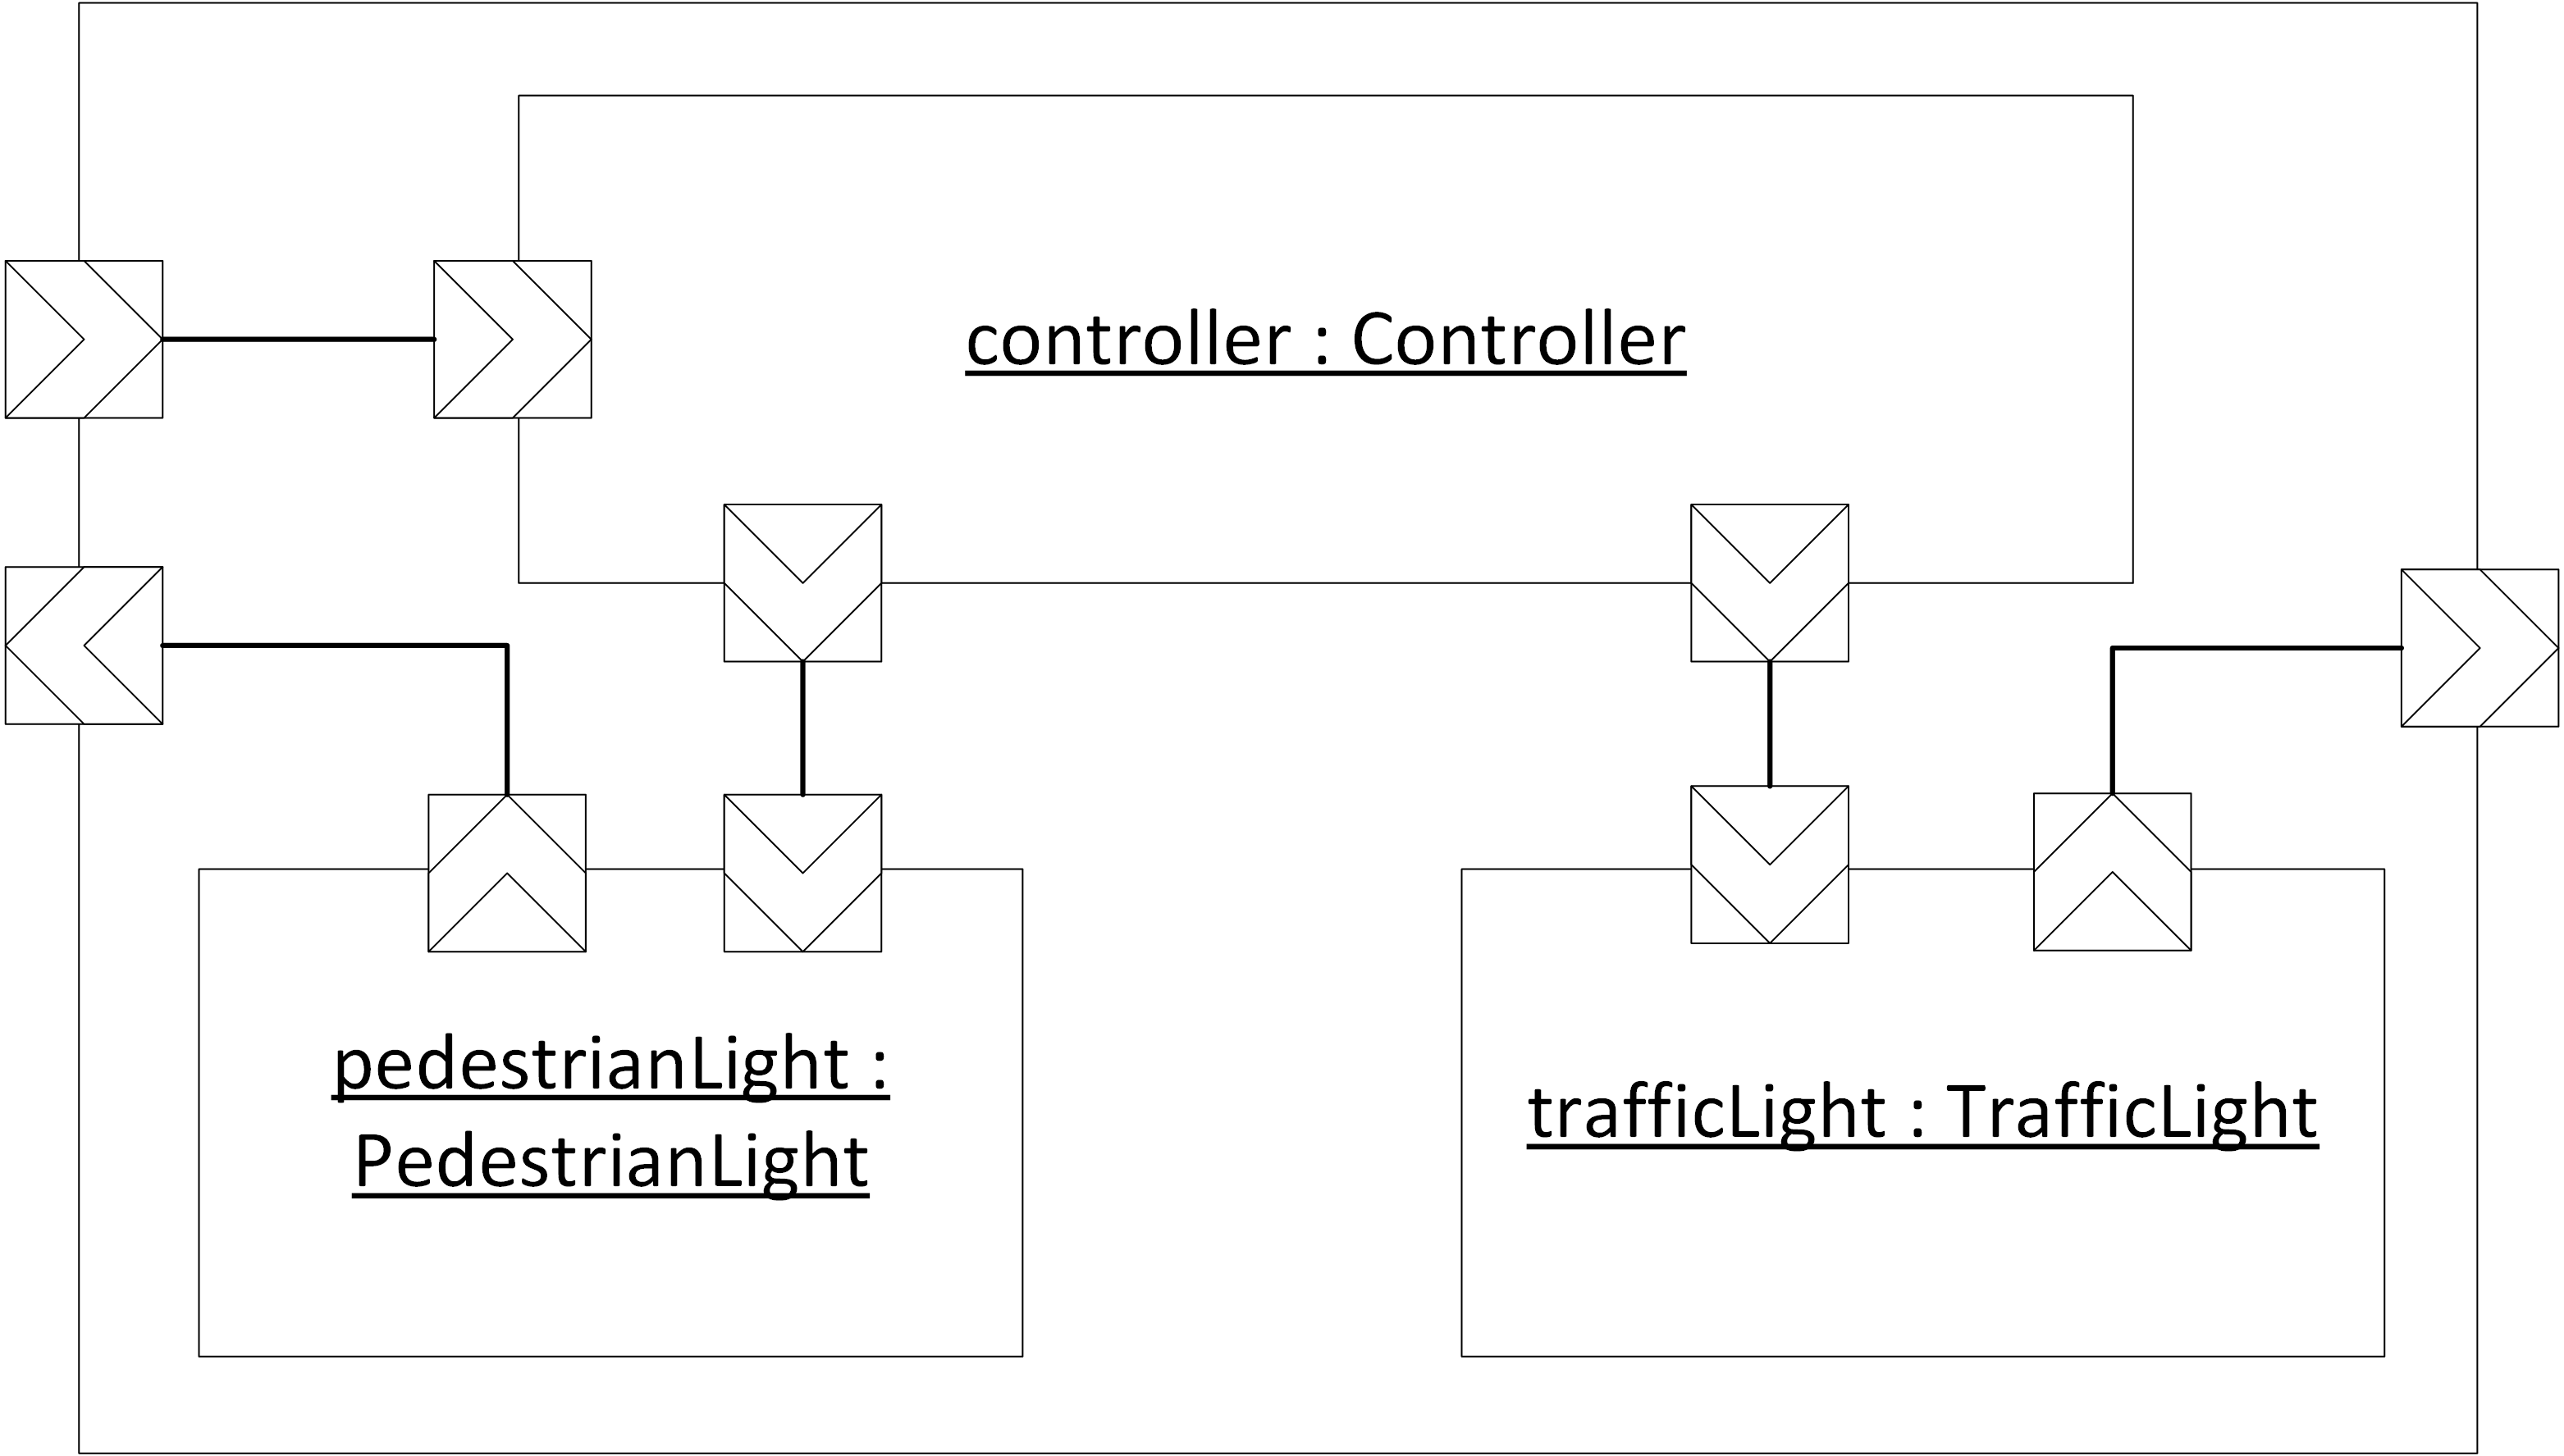
\includegraphics[width=130mm, keepaspectratio]{figures/casestudy_blockdiagram.png}
	%}
	\caption{Components of the modeled system and their connections} 
	\label{fig_casestudy_blockdiagram}
\end{figure}

\textbf{The Expected Behavior of the Components} 

The components have been separated and their interfaces precisely defined, thus, we can proceed to formulating behavior-related requirements. For instance, the traffic light component must conform to the following -- not exhaustive -- list:

\begin{itemize}
	\item The traffic light must loop through the sequence 'toggle/red toggle/green toggle/yellow toggle/red' during normal operation.
	\item The traffic light must display blinking yellow signal when a police interrupt arrives during normal operation.
	\item The traffic light must return to normal operation when a second interrupt arrives.
	\item The traffic light must display red signal when returning to normal operation.
	\item The traffic light must always display blinking yellow when interrupted. 

\end{itemize}

A very similar list can be constructed for the pedestrian light component. The controller component is slightly more complicated, as it may toggle or interrupt the other components at the same time, so its alphabet shall contain separate elements for these cases.

%---------------------------------------------------------------
\subsection{Synthesizing the Components} \label{subs_casestudysynth}
%---------------------------------------------------------------

Now we add the previously formulated requirements to the ILE, in formalisms that it is able to interpret. In the following examples for the interaction of the user with the ILE, '$\circ$' symbolizes the ILE and '$\triangleright$' symbolizes the user (interface qualifications are omitted for shorter and simpler expressions). 

\bigskip
\fbox{
	\parbox{\textwidth}{
		\begin{itemize}
			\setlength\itemsep{0.2em}
			\item[$\circ$] Provide the requirements for component 'TrafficLight':
			\item[$\triangleright$] Valid Trace: toggle/red toggle/green toggle/yellow toggle/red
			\item[$\triangleright$] LTL Expression: F(interrupt -> X(G(toggle) -> G(blinkingYellow)))
			\item[$\triangleright$] Invalid Trace: interrupt/red interrupt/blinkingYellow
			\item[$\triangleright$] LTL Expression: F(G(interrupt -> (blinkingYellow | red)))
			
			\smallskip
			... other components ...
		\end{itemize}
	}
}

\bigskip
After adding these requirements during the offline phase, the synthesis of the components can proceed to the online, interactive phase. A possible run of the learning process can be seen below.

\bigskip
\fbox{
	\parbox{\textwidth}{
		\begin{itemize}
			\setlength\itemsep{0.2em}
			\item[$\circ$] Learning component 'TrafficLight'
			\item[$\circ$] Provide the output for sequence [toggle, interrupt]:
			\item[$\triangleright$] Corresponding Output: blinkingYellow
			\item[$\circ$] Provide the output for sequence [toggle, interrupt, interrupt]:
			\item[$\triangleright$] Corresponding Output: red
			\item[$\circ$] Provide the output for sequence [toggle, toggle, interrupt]:
			\item[$\triangleright$] Corresponding Output: blinkingYellow
			\item[$\circ$] Provide the output for sequence [toggle, toggle, interrupt, interrupt]:
			\item[$\triangleright$] Corresponding Output: red
			\item[$\circ$] Provide the output for sequence [toggle, toggle, toggle, interrupt]:
			\item[$\triangleright$] Corresponding Output: blinkingYellow
			\item[$\circ$] Equivalence Query (Figure \ref{fig_trafficlightincomplete} in the Appendix)
			\item[$\triangleright$] Counterexample: interrupt interrupt
			\item[$\circ$] Provide the output for sequence [interrupt, interrupt, interrupt]:
			\item[$\triangleright$] Valid Trace: interrupt/blinkingYellow interrupt/red interrupt/blinkingYellow interrupt/red
			\item[$\circ$] Provide the output for sequence [interrupt, interrupt, toggle]:
			\item[$\triangleright$] Corresponding Output: green
			\item[$\circ$] Provide the output for sequence [interrupt, toggle, interrupt]:
			\item[$\triangleright$] Corresponding Output: red
			\item[$\circ$] Equivalence Query (Figure \ref{fig_casestudy_trafficlightlearned})
			\item[$\triangleright$] Approved.
			
			\smallskip
			... other components ...
		\end{itemize}
	}
}

\bigskip
The same learning process can be seen on Listing \ref{lst_examplelearning} in the Appendix, which presents the inputs and outputs as they appeara on the command line interface.

%---------------------------------------------------------------
\subsection{The Learned Models} \label{subs_casestudyresults}
%---------------------------------------------------------------

Now we can examine any differences between the expected and the learned models. Figure \ref{fig_casestudy_trafficlightdiff} presents the expected and the synthesized traffic light models.

\begin{figure}[!ht] 
	\centering
	\begin{subfigure}[b]{0.9\textwidth}
		\centering
		\fbox{
			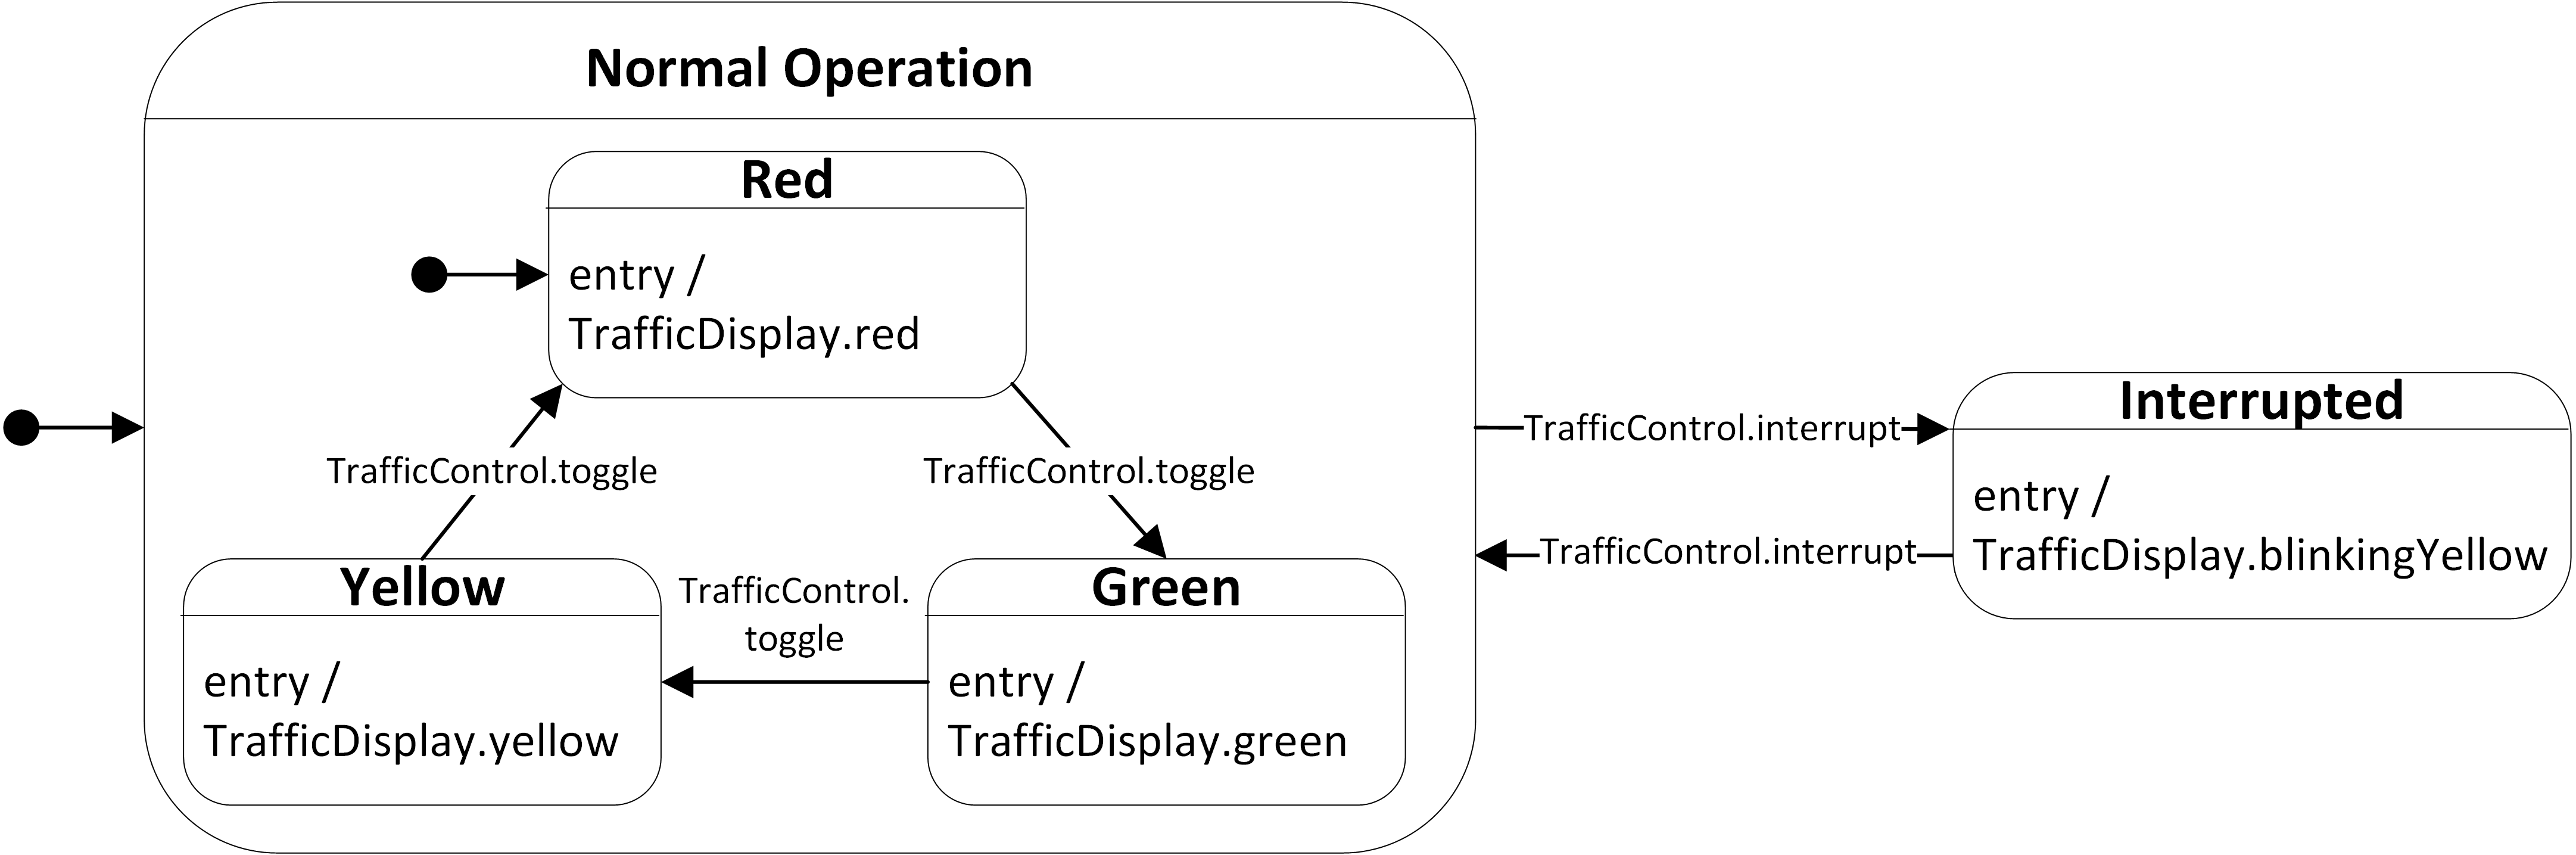
\includegraphics[width=120mm]{figures/casestudy_trafficlightexpected.png}
		}	
		\caption{Expected}
	\end{subfigure}
	\hfill
	\begin{subfigure}[b]{0.9\textwidth}
		\centering
		\fbox{
			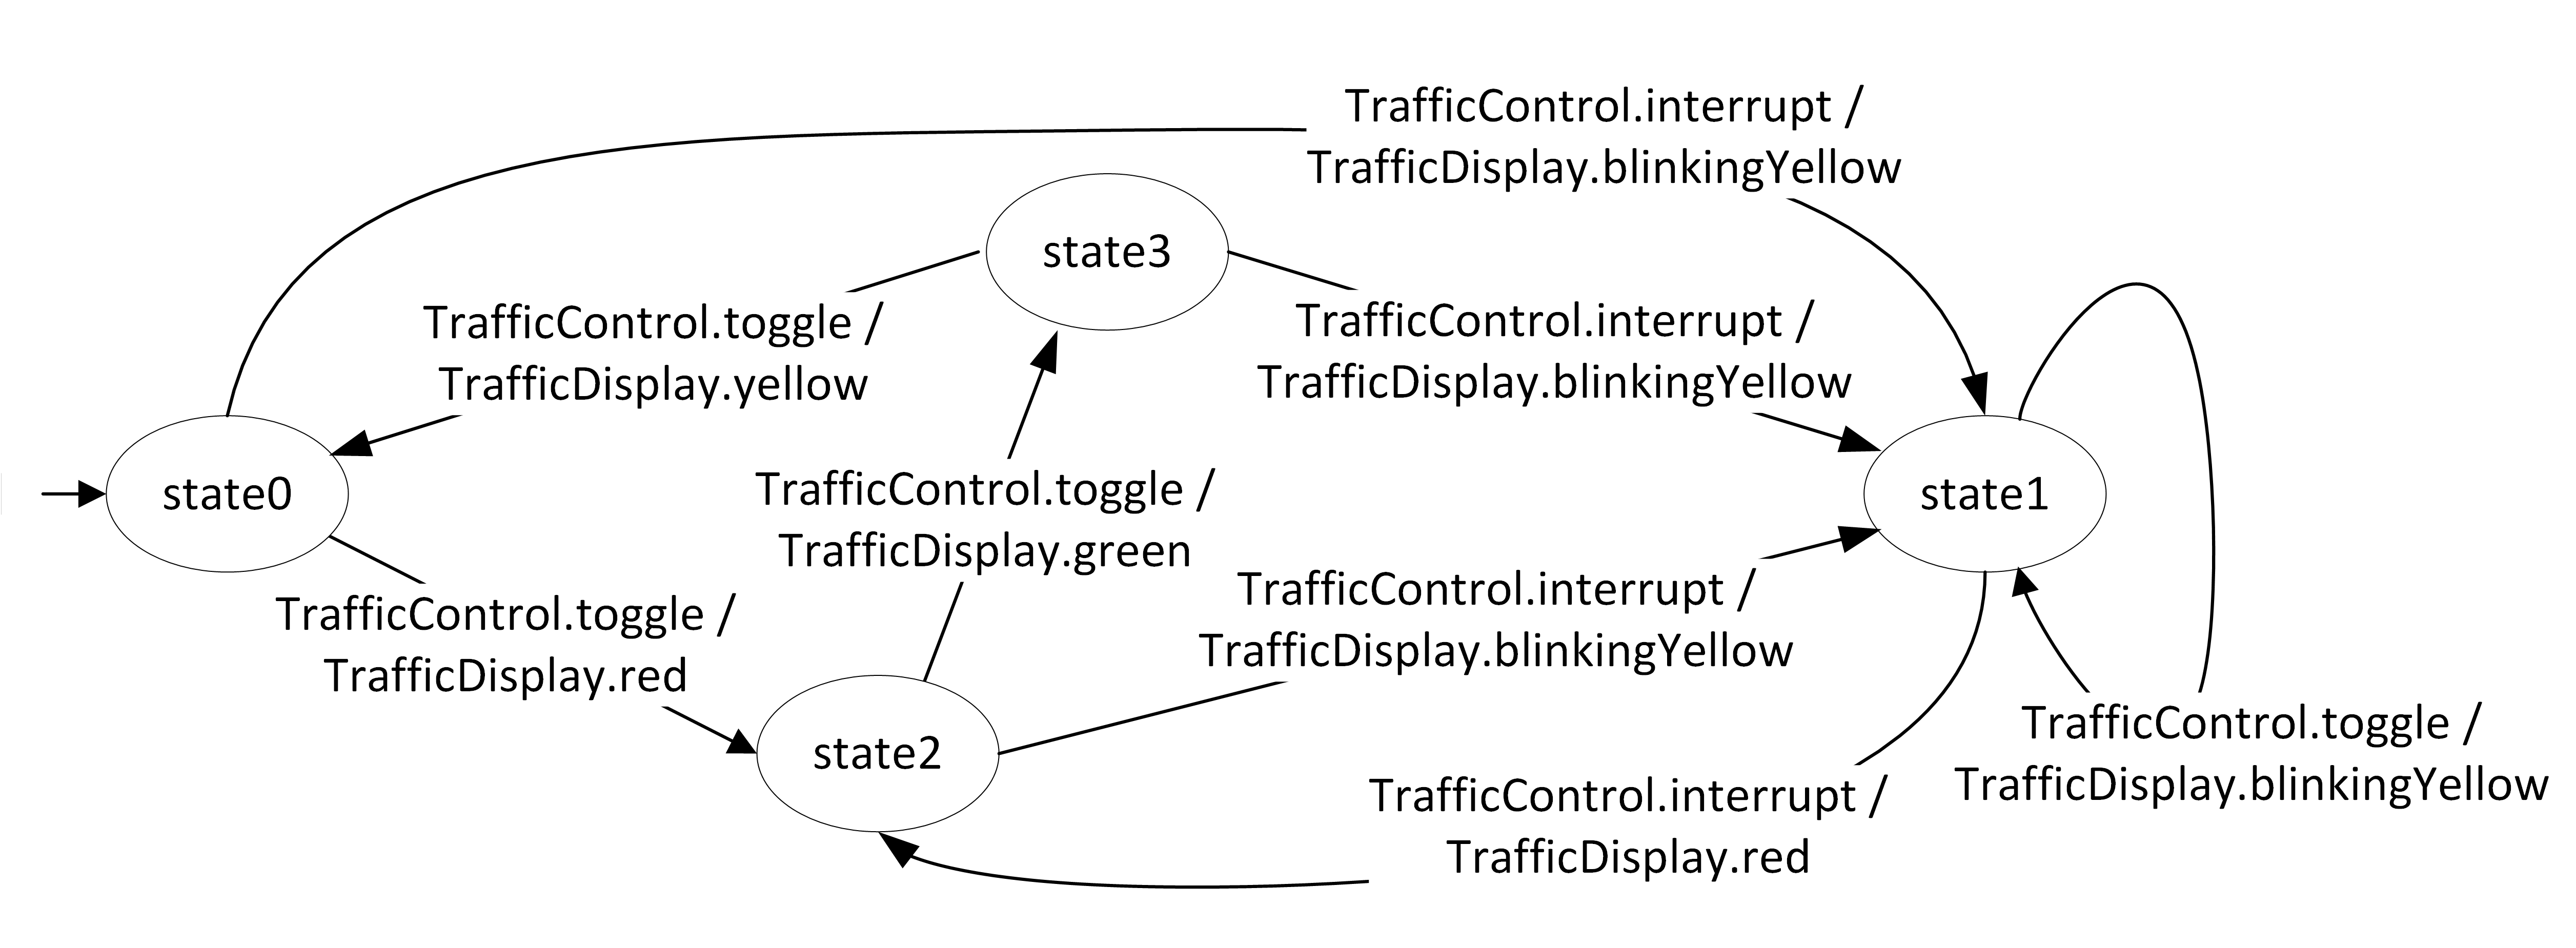
\includegraphics[width=120mm]{figures/casestudy_trafficlightlearned.png}
		}
		\caption{Learned}	
		\label{fig_casestudy_trafficlightlearned}
	\end{subfigure}
	\caption{The expected and the learned traffic light components}
	\label{fig_casestudy_trafficlightdiff}
\end{figure}

The structure of the models is clearly different, notably:
\begin{itemize}
	\item The expected models contain hierarchical states, while the learned ones are 'flat'.
	\item The expected models also contain entry and exit actions, while the learned models only contain actions on transitions. 
	\item The expected models contain meaningful state names, while the learned ones only have generated ones.
\end{itemize}

However, the models are behaviorally equivalent. Both models meet the requirements stated in Subsection \ref{subs_casestudycomps}, and after careful examination, it is obvious that the only initial states are different -- as no entry actions are used in the learned models -- and the transition starting from the hierarchical state is separated into three different transitions.

The differences between the expected and learned pedestrian light components can be seen on Figure \ref{fig_casestudy_pedestrianlightdiff}. The differences are the similar to those of the traffic light models, as the modeled behavior is also very similar. 

\begin{figure}[!ht] 
	\centering
	\begin{subfigure}[b]{0.9\textwidth}
		\centering
		\fbox{
			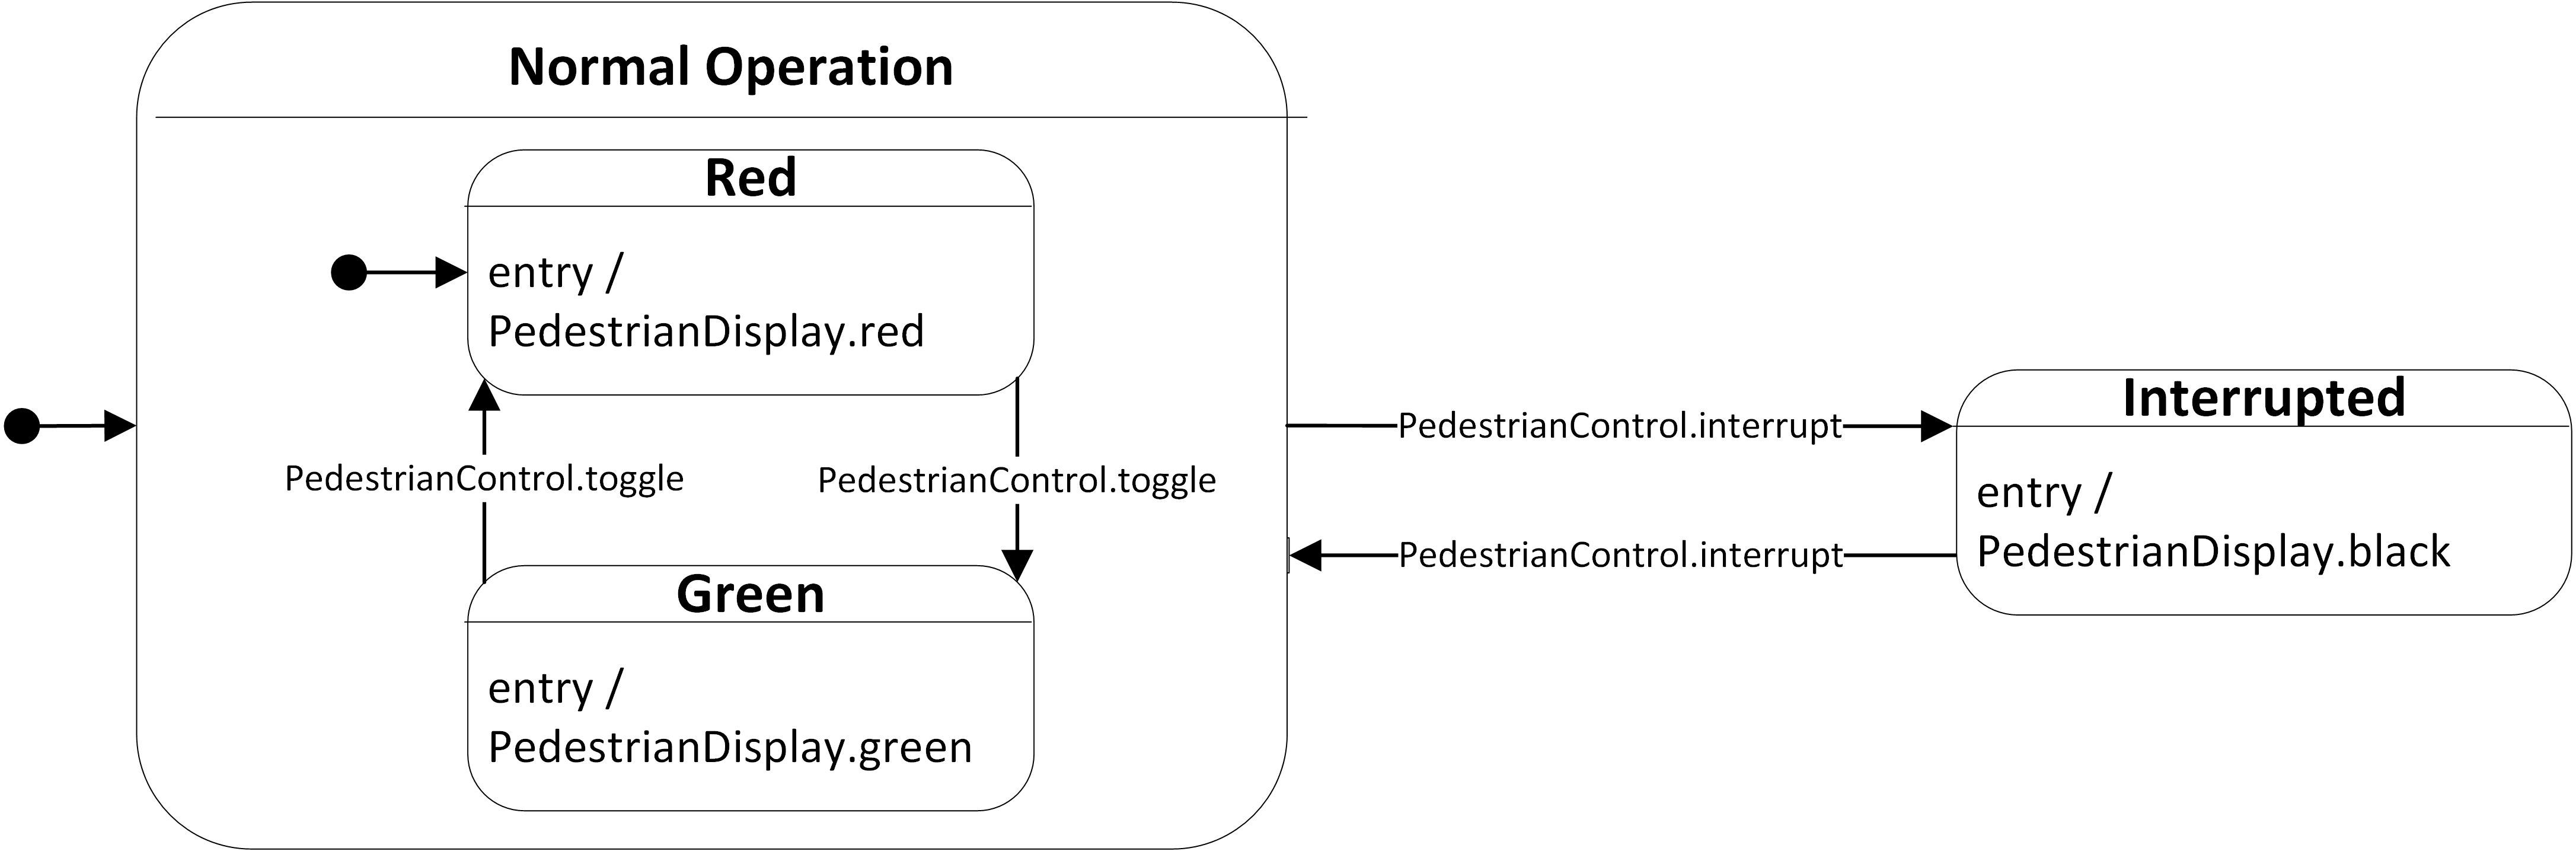
\includegraphics[width=120mm]{figures/casestudy_pedestrianlightexpected.png}
		}	
		\caption{Expected}
	\end{subfigure}
	\hfill
	\begin{subfigure}[b]{0.9\textwidth}
		\centering
		\fbox{
			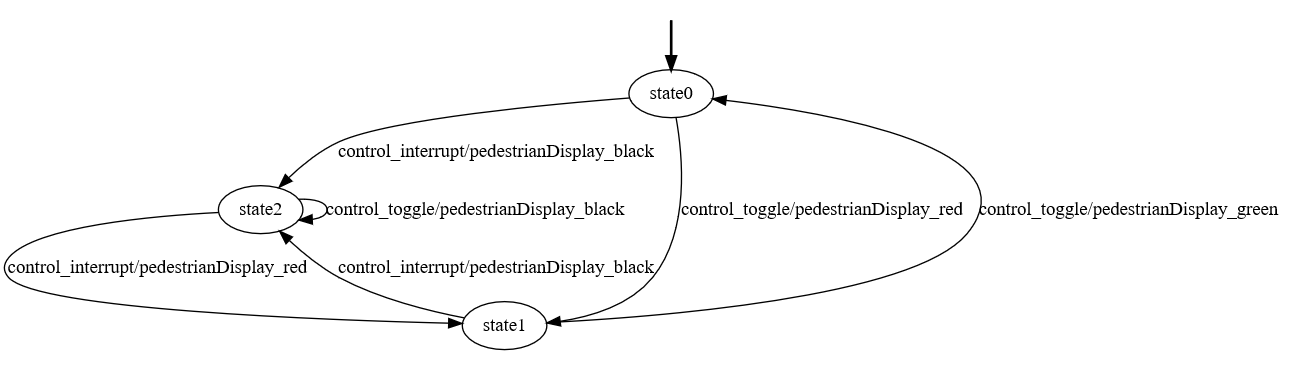
\includegraphics[width=120mm]{figures/casestudy_pedestrianlightlearned.PNG}
		}
		\caption{Learned}	
	\end{subfigure}
	\caption{The expected and the learned pedestrian light components}
	\label{fig_casestudy_pedestrianlightdiff}
\end{figure}

The behavior of the controller component can be learned similarly. The expected and the synthesized models can be seen on Figure \ref{fig_casestudy_controllerdiff}. Note, that in addition to '{\fontfamily{qcr}\selectfont Police.interrupt}', the component also has an unqualified t input word. This represents a timeout event the engineer must extend the serialized model with -- but acts as a regular input event during the learning. 

\begin{figure}[!ht] 
	\centering
	\begin{subfigure}[b]{0.9\textwidth}
		\centering
		\fbox{
			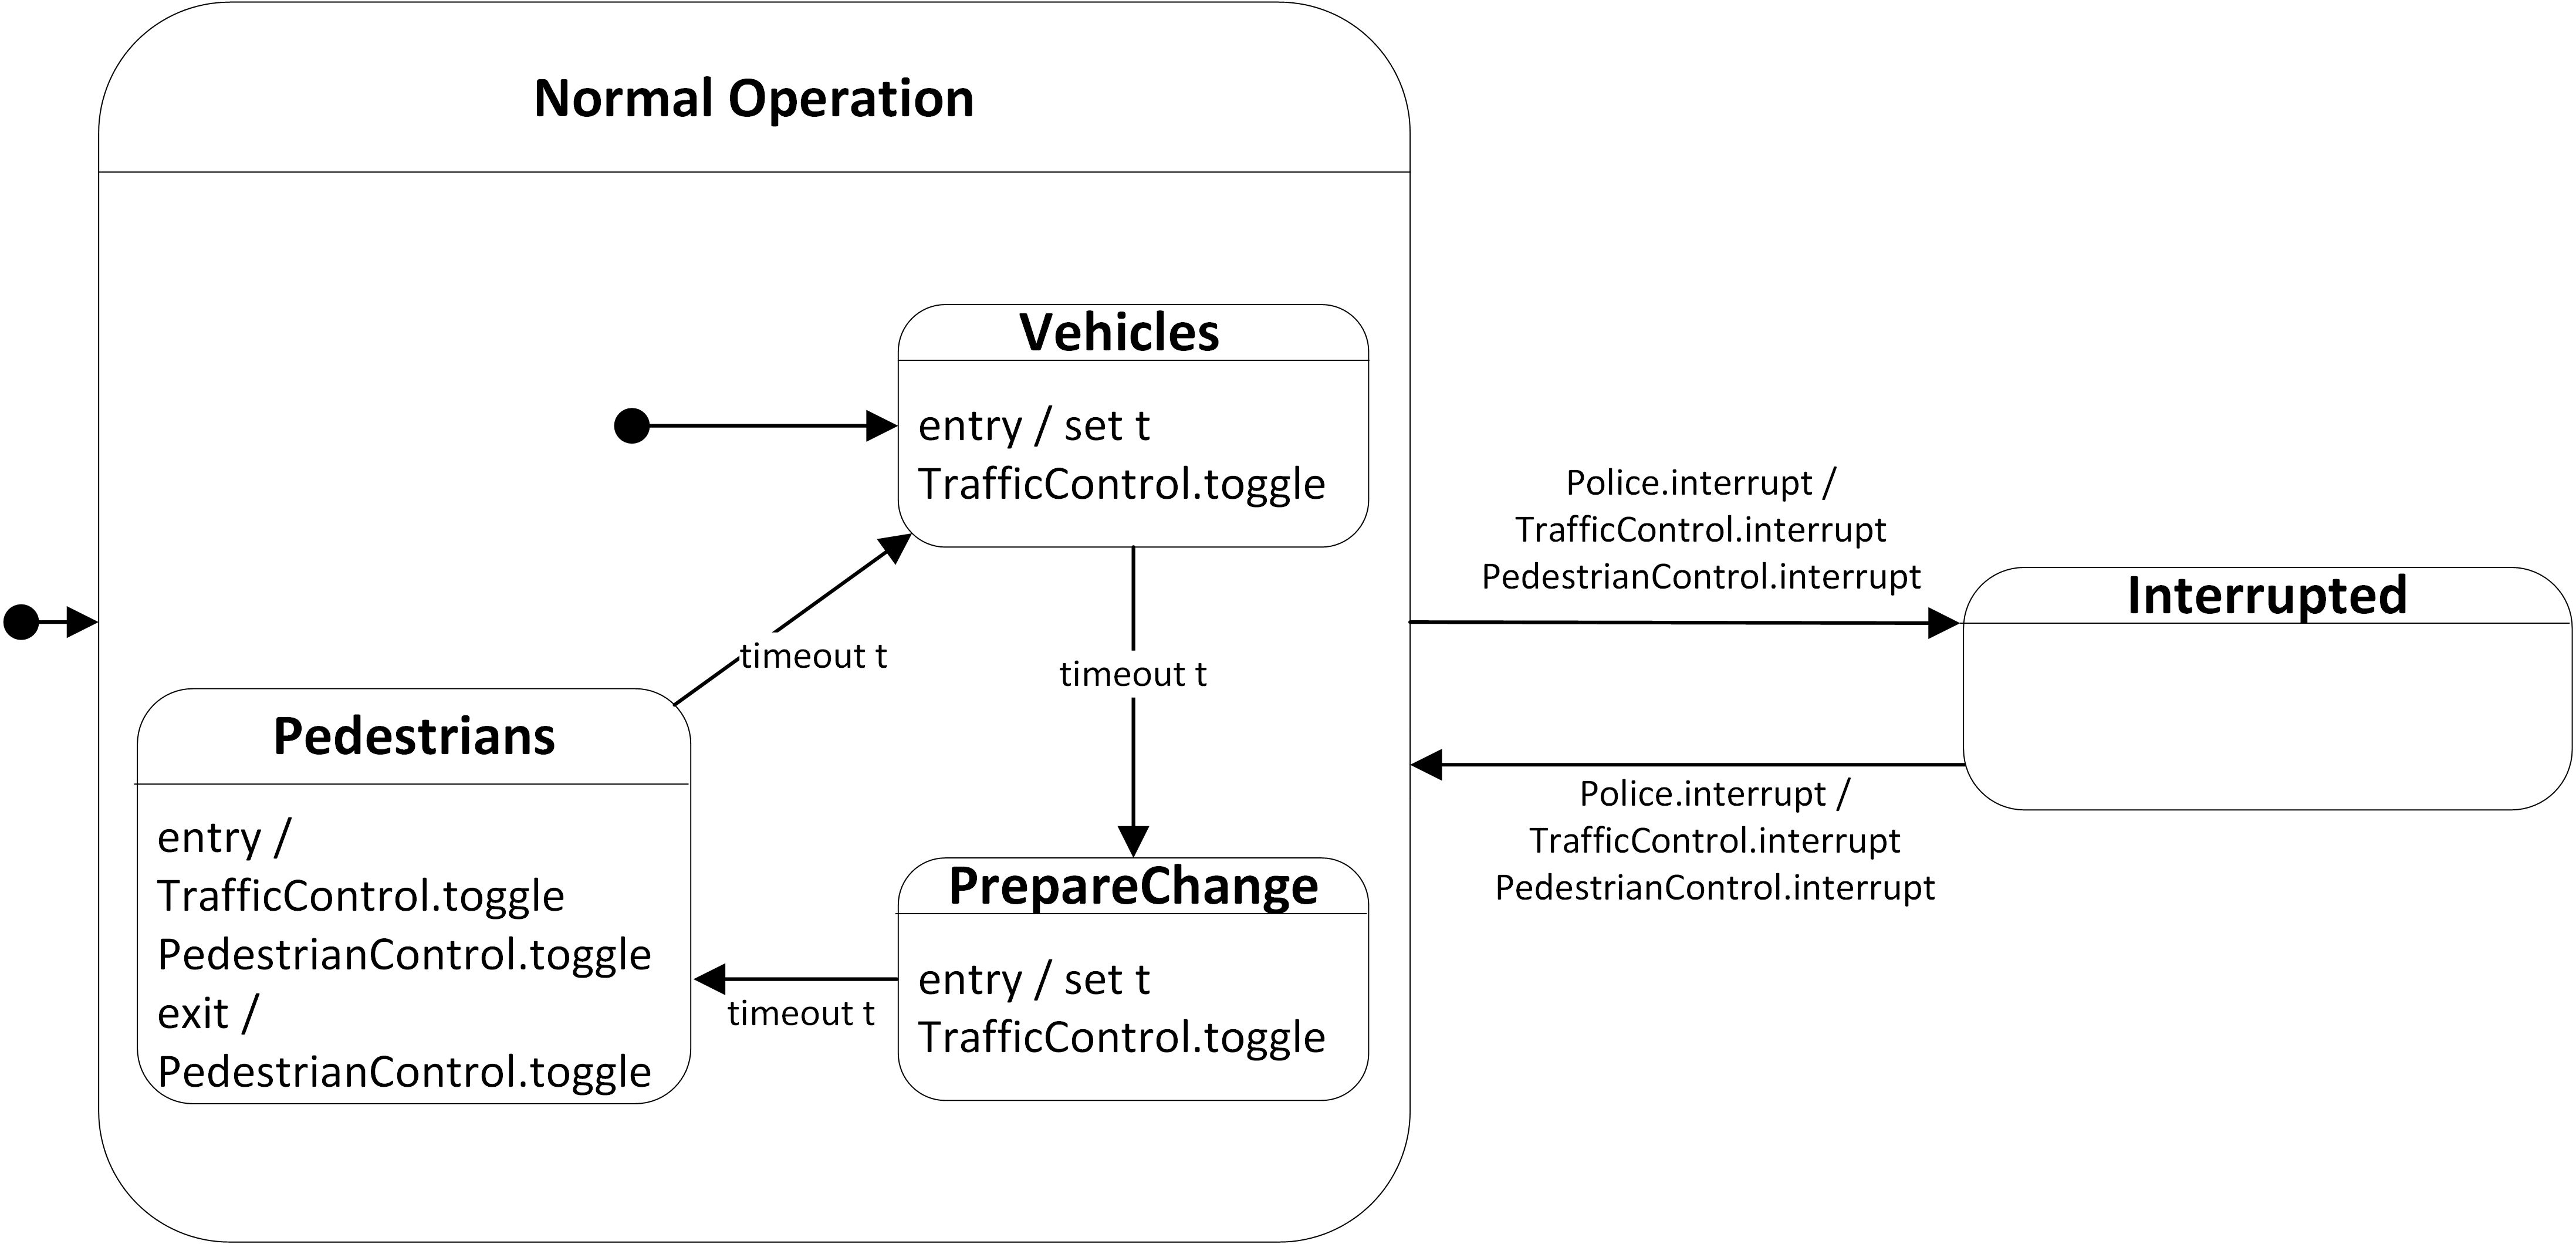
\includegraphics[width=120mm]{figures/casestudy_controllerexpected.png}
		}	
		\caption{Expected}
	\end{subfigure}
	\hfill
	\begin{subfigure}[b]{0.9\textwidth}
		\centering
		\fbox{
			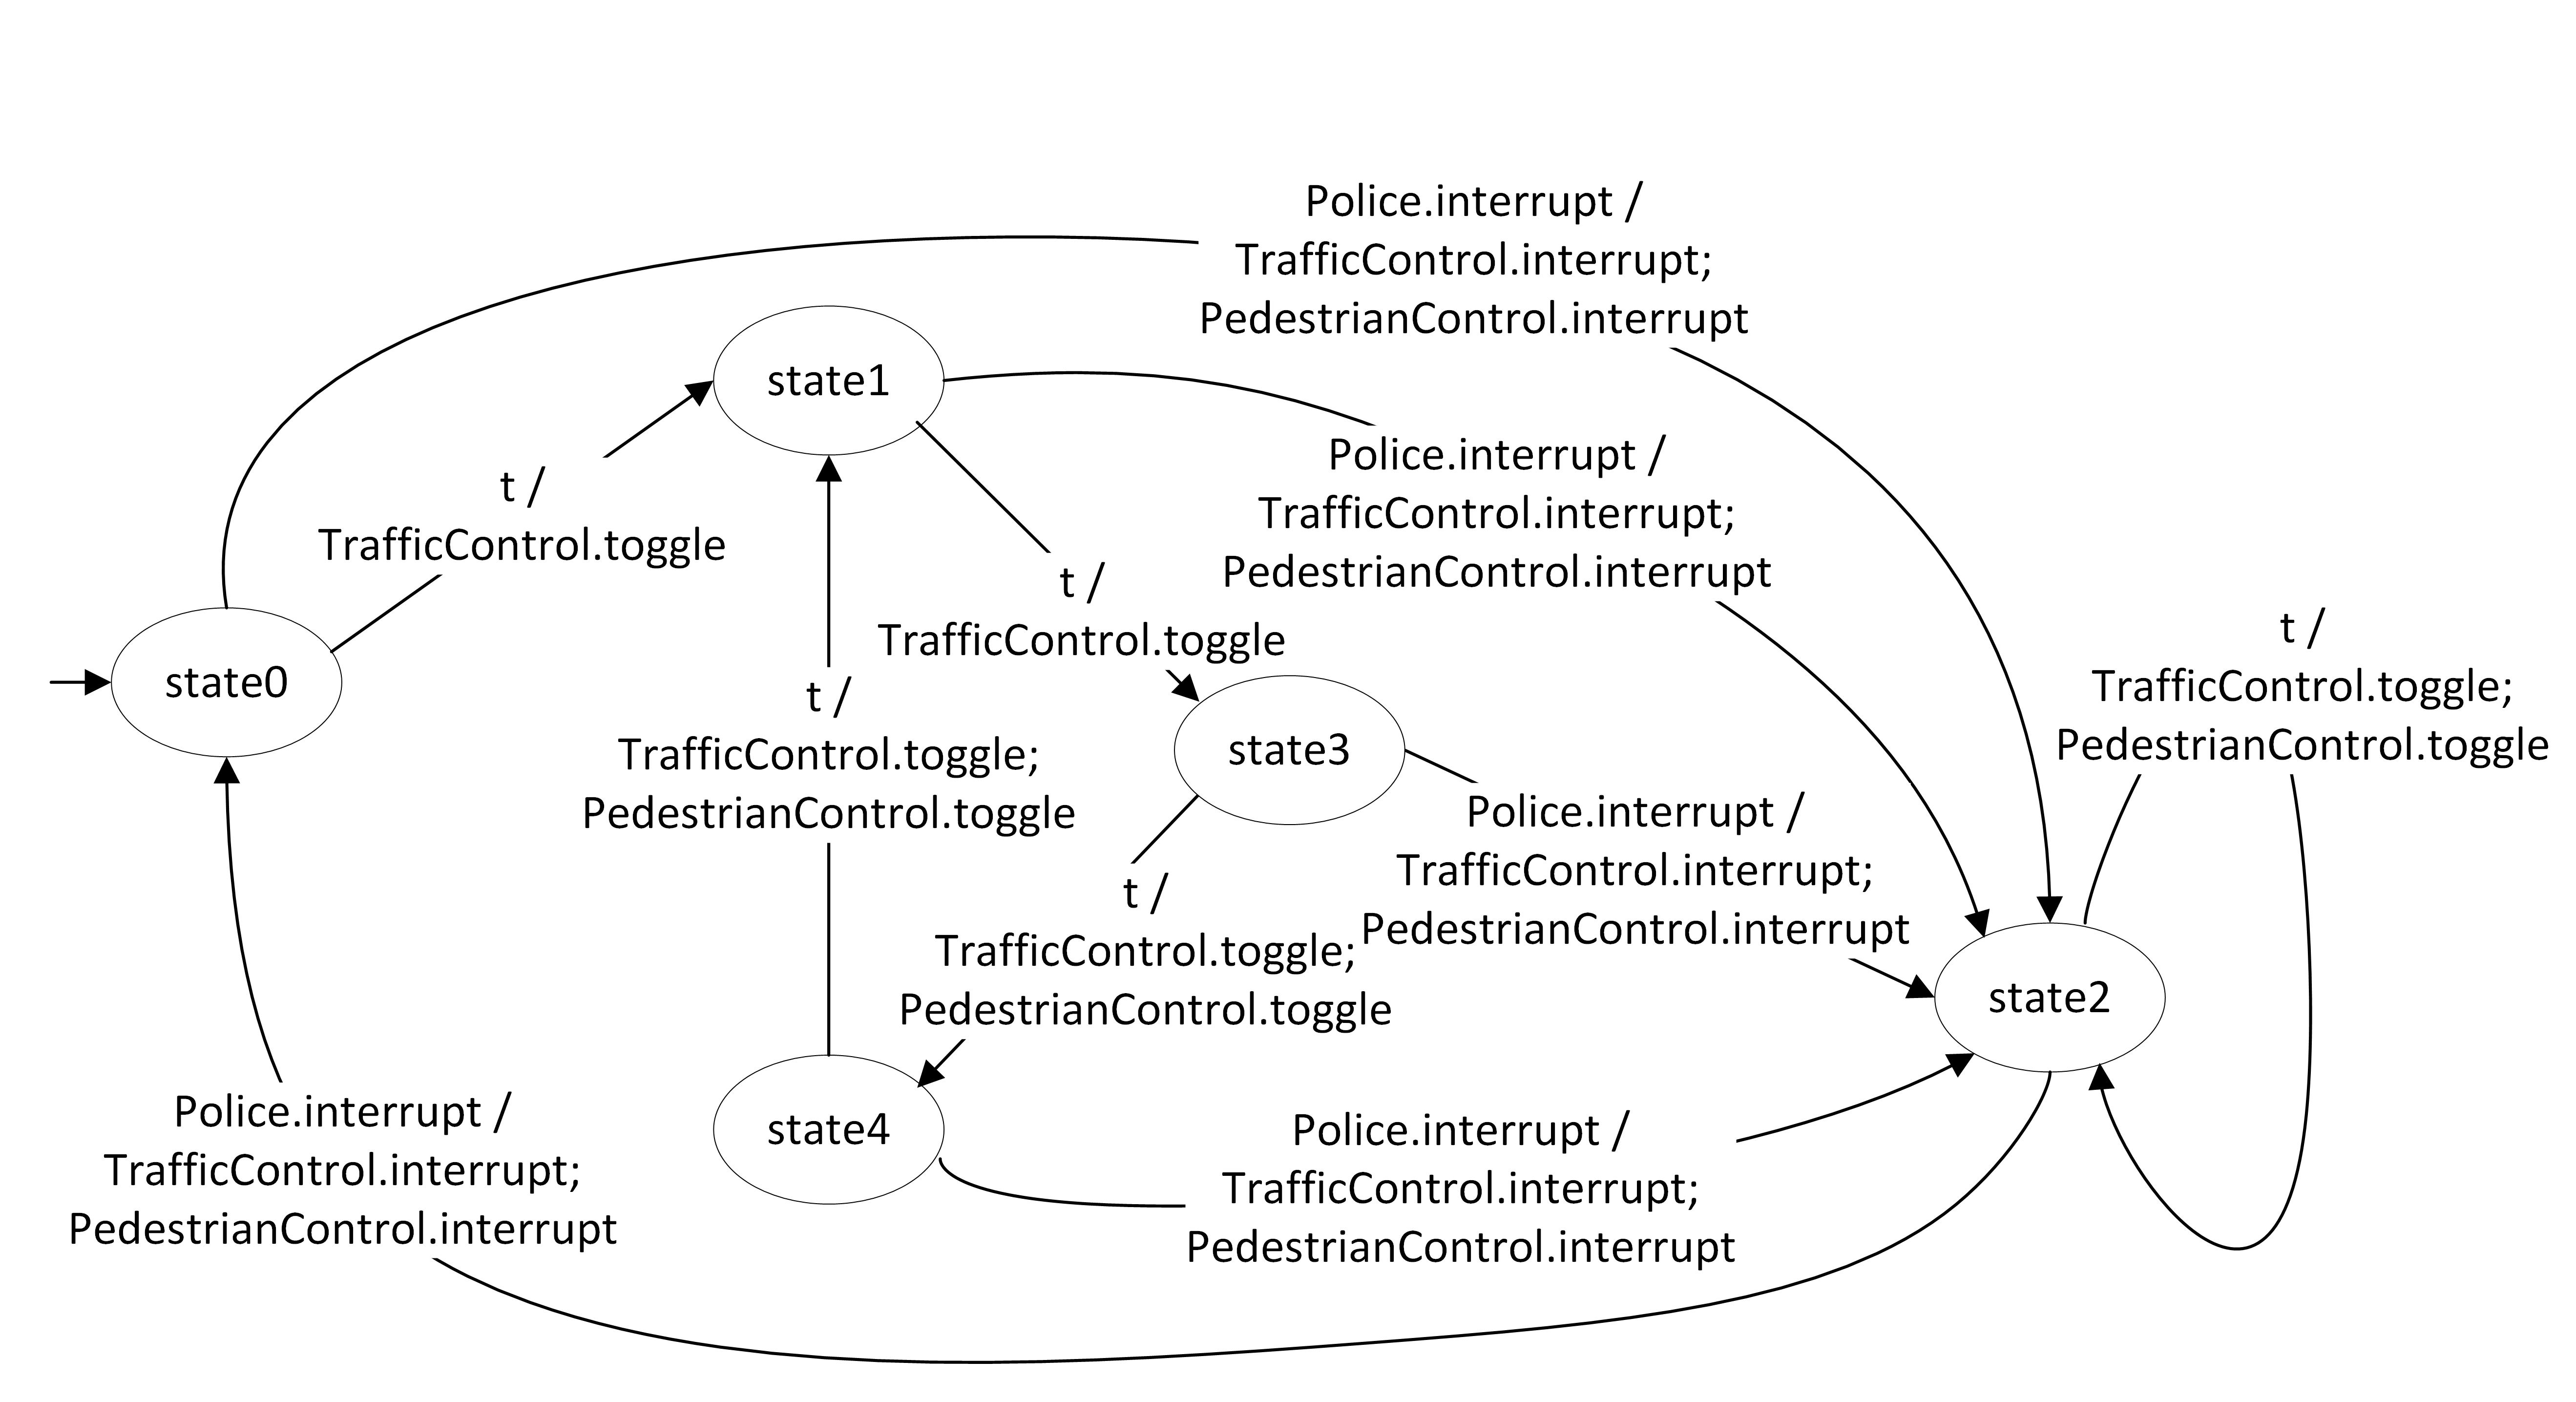
\includegraphics[width=120mm]{figures/casestudy_controllerlearned.png}
		}
		\caption{Learned [TODO ezt szebbre]}	
	\end{subfigure}
	\caption{The expected and the learned controller components}
	\label{fig_casestudy_controllerdiff}
\end{figure}

After learning every component, the collection of the models is serialized as a Gamma project, with the following files and contents:
\begin{itemize}
	\item TrafficLight.gcd (the learned traffic light component)
	\item PedestrianLight.gcd (the learned pedestrian light component)
	\item Controller.gcd (the learned controller component)
	\item CompositeSystem.gcd (connections between the component ports, as illustrated on Figure \ref{fig_casestudy_blockdiagram})
	\item Interfaces.gcd (the interface definitions based on the ports of the components)
\end{itemize}
After extending the controller with statechart-specific elements (namely the timeout event), the engineer can use the Gamma Framework to check the correctness of the system model or even generate implementation code.


[TODO ESETLEG: a teljes rendszert is tanuljuk?]

\clearpage
%----------------------------------------------------------------------------
\section{Theoretical Evaluation} \label{sec_theoeval}
%----------------------------------------------------------------------------
%TODO: Bevezető

%---------------------------------------------------------------
\subsection{The Oracle} \label{subs_evaloracle}
%---------------------------------------------------------------
%TODO: Optimistic vs Pessimistic, formalizmusok
%TODO review and update figure and its caption
The main metric of the oracle is the number of questions the engineer has to answer during the course of the model synthesis. This is really difficult to measure, as the exact number of these questions depends on multiple parameters: the complexity of the desired model, as well as the order, formalism, complexity and skillful construction of the requirements formulated by the designing engineer. Some of these parameters is difficult to measure in itself, thus, the following measurement is rather an illustration of the capabilities of the framework through a realistic example. 

For this, the traffic light component from the case study in Section \ref{sec_casestudy} is going to be used. We assume, that the user only adds requirements he perceives conducive to the model synthesis and tries to formulate realistic -- not unnecessarily complex -- requirements. 

The baseline of this experiment is the number of questions the user has to answer by always providing the corresponding outputs to the questions of the ILE, as higher numbers are the result of unnecessary information. Then, we are going to examine the cases when valid traces are also allowed, then add LTL expressions and finally invalid traces. Sequence diagrams are excluded from these measurements. The results can be seen on Figure \ref{fig_eval_trafficlightformalisms}.

\begin{figure}[!ht] 
	\centering
	%\fbox{
	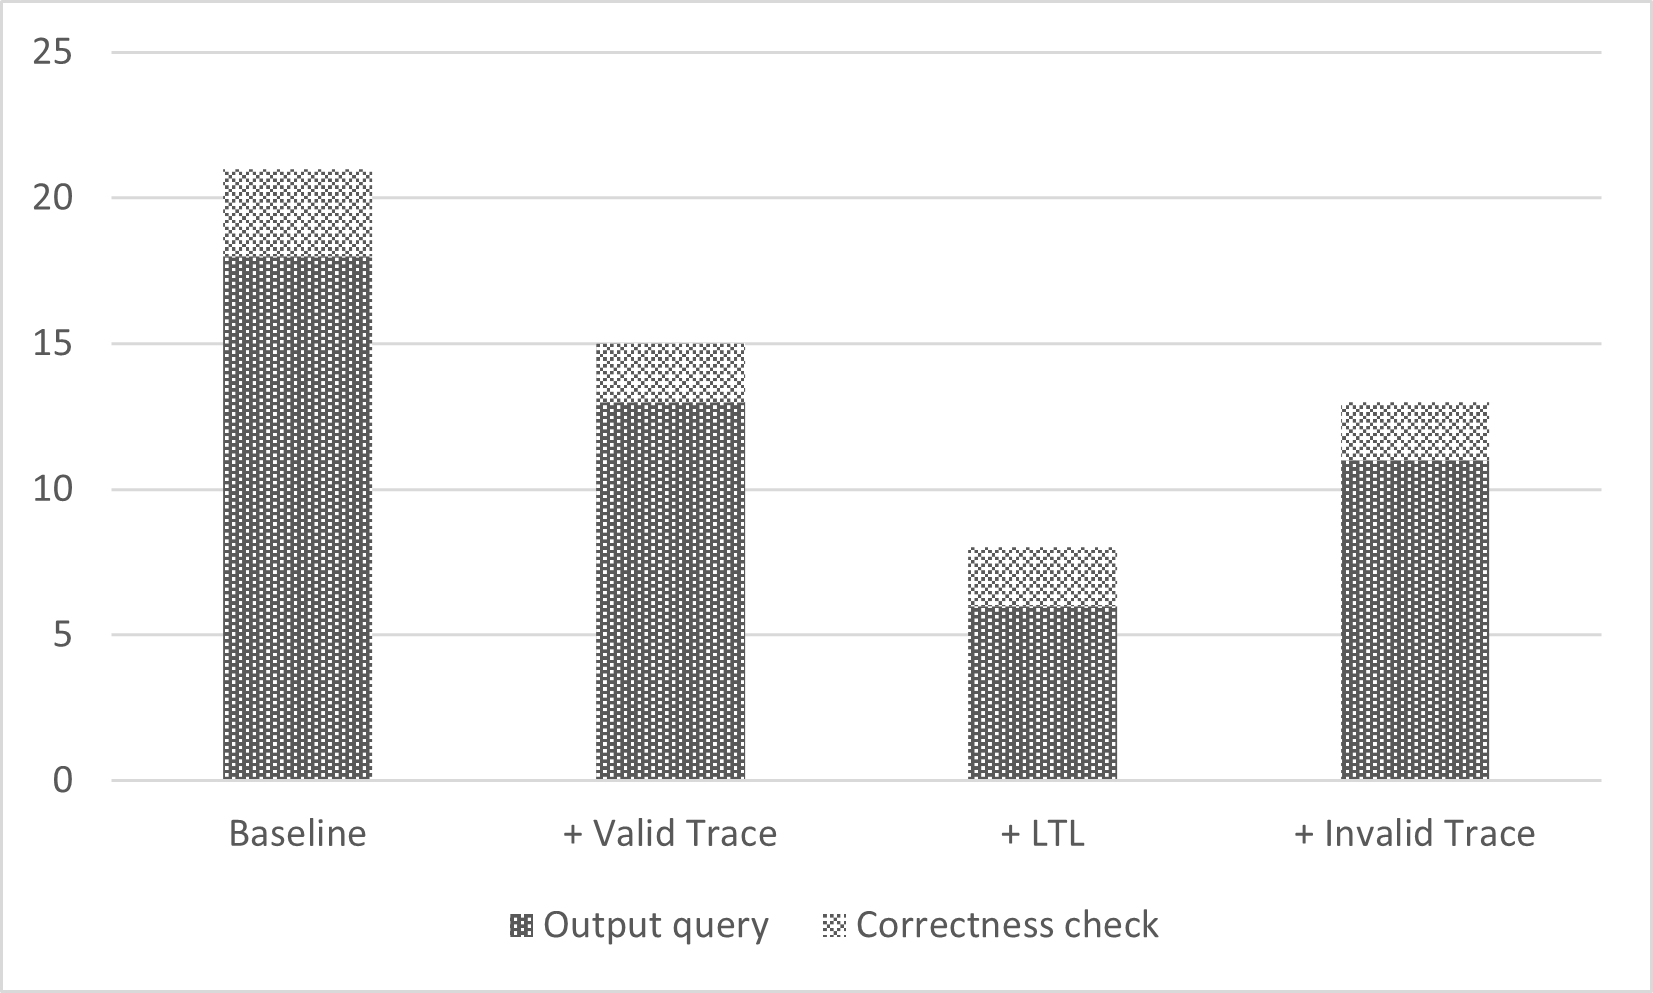
\includegraphics[width=130mm, keepaspectratio]{figures/evaluation_trafficlightformalism.png}
	%}
	\caption{Components of the modeled system and their connections} 
	\label{fig_eval_trafficlightformalisms}
\end{figure}

The requirements used in this experiment -- apart from the corresponding outputs answering the questions of the ILE directly -- can be seen in [TODO appendix]. The smallest number of queries was measured when both valid traces and LTL expressions were used. The addition of invalid traces resulted in a slightly higher number, demonstrating that this formalism is difficult to apply and useful mostly for its other benefits.  
 
%---------------------------------------------------------------
\subsection{The Learning Algorithm} \label{subs_evallearningalgo}
%---------------------------------------------------------------
%TODO: Optimistic vs Pessimistic, minimization

%---------------------------------------------------------------
\subsection{Caching} \label{subs_evalcaching}
%---------------------------------------------------------------
%TODO: optimisticre mennyit csökkent, RESET